\section{Agrupamento de fases}

\begin{frame}[fragile]{Interface de vanguarda}

    \begin{itemize}
        \item Na práticas, as fases de um compilador são agrupadas em duas interfaces: vanguarda e retaguarda
       %\pause

        \item A interface de vanguarda contém as fases que dependem primariamente do programa fonte e que independem da máquina alvo
       %\pause

        \item Em geral, ela inclui as fases de análise, a criação da tabela de símbolos e a geração de código intermediário
       %\pause

        \item Ela também inclui o tratamento de erros associados a estas fases
       %\pause

        \item Embora a otimização faça parte primariamente da interface de retaguarda, é possível aplicar algum nível de otimização na interface de
        vanguarda
    \end{itemize}

\end{frame}

\begin{frame}[fragile]{Interface de retaguarda}

    \begin{itemize}
        \item A interface de retaguarda contém as fases que dependem primariamente da máquina alvo, e independem do programa fonte
       %\pause

        \item O ponto de partida é o código intermediário
       %\pause

        \item Assim, esta interface contém, em geral, as fases de otimização e geração de código
       %\pause

        \item Ela também manipula a tabela de símbolos e trata dos erros associados à estas últimas duas fases
       %\pause

        \item No cenário ideal, ambas interfaces são independentes, o que permite fixar uma delas e alterar a outra para obter diferentes compiladores com
        diferentes objetivos
    \end{itemize}

\end{frame}

\begin{frame}[fragile]{Compiladores de uma mesma linguagem para múltiplas máquinas}

    \begin{figure}
        \centering 

        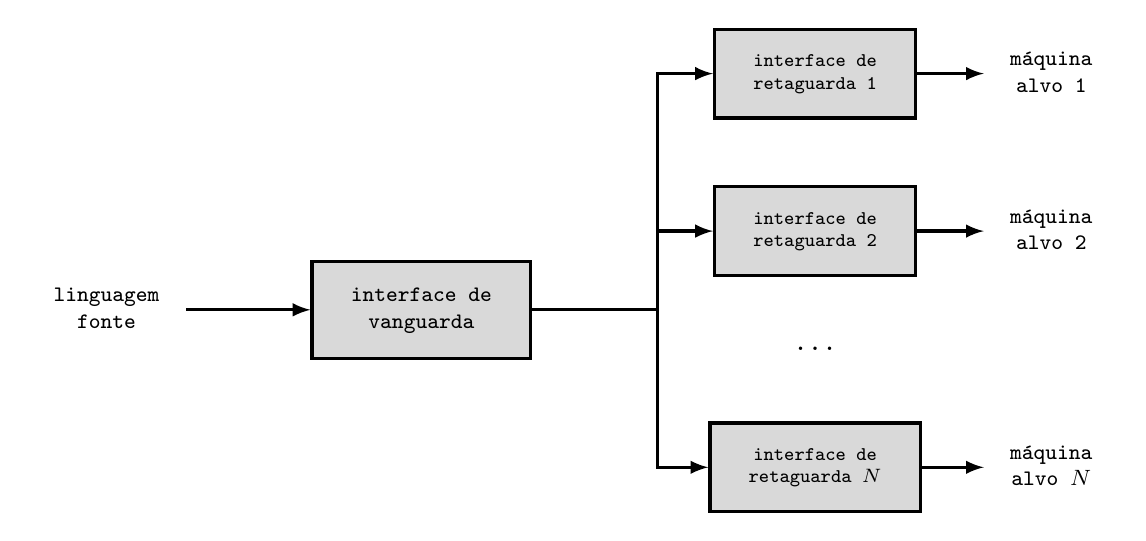
\begin{tikzpicture}

            \node[draw,very thick,fill=gray!30,inner sep=8pt] (Y) at (4, 3) { \footnotesize \begin{tabular}{c}\texttt{interface de}\\ \texttt{vanguarda}\end{tabular} };
            \node[draw,very thick,fill=gray!30,inner sep=8pt] (A) at (9, 6) { \scriptsize \begin{tabular}{c}\texttt{interface de}\\ \texttt{retaguarda 1}\end{tabular} };
            \node[draw,very thick,fill=gray!30,inner sep=8pt] (B) at (9, 4) { \scriptsize \begin{tabular}{c}\texttt{interface de}\\ \texttt{retaguarda 2}\end{tabular} };
            \node (C) at (9, 2.5) { \texttt{...} };

            \node[draw,very thick,fill=gray!30,inner sep=8pt] (D) at (9, 1) { \scriptsize \begin{tabular}{c}\texttt{interface de}\\ \texttt{retaguarda $N$}\end{tabular} };

            \node (X) at (0, 3) { \footnotesize \begin{tabular}{c}\texttt{linguagem}\\ \texttt{fonte}\end{tabular} };
            \node (Z1) at (12, 6) { \footnotesize \begin{tabular}{c}\texttt{máquina}\\ \texttt{alvo 1}\end{tabular} };
            \node (Z2) at (12, 4) { \footnotesize \begin{tabular}{c}\texttt{máquina}\\ \texttt{alvo 2}\end{tabular} };
            \node (Z3) at (12, 1) { \footnotesize \begin{tabular}{c}\texttt{máquina}\\ \texttt{alvo $N$}\end{tabular} };

            \coordinate (P) at (7, 3);
            \coordinate (P1) at (7, 6);
            \coordinate (P2) at (7, 4);
            \coordinate (P3) at (7, 1);

            \draw[very thick,latex-] (Y) to (X);
            \draw[very thick,-latex] (Y) to (P) to (P1) to (A);
            \draw[very thick,-latex] (Y) to (P) to (P2) to (B);
            \draw[very thick,-latex] (Y) to (P) to (P3) to (D);
            \draw[very thick,-latex] (A) to (Z1);
            \draw[very thick,-latex] (B) to (Z2);
            \draw[very thick,-latex] (D) to (Z3);

        \end{tikzpicture}
    \end{figure}

\end{frame}

\begin{frame}[fragile]{Compiladores de múltiplas linguagens para uma mesma máquina}

    \begin{figure}
        \centering 

        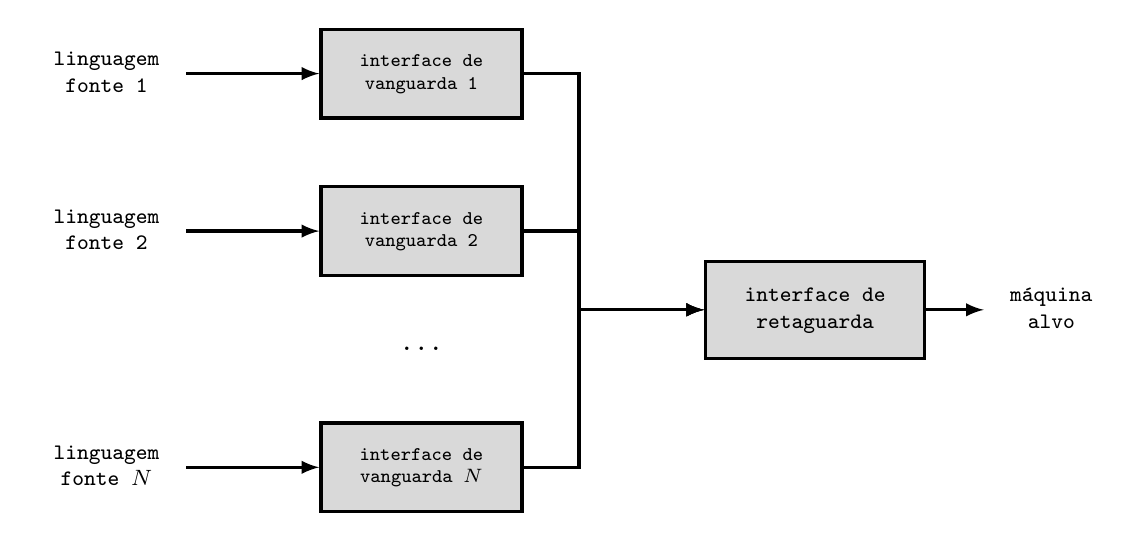
\begin{tikzpicture}

            \node[draw,very thick,fill=gray!30,inner sep=8pt] (Y) at (9, 3) { \footnotesize \begin{tabular}{c}\texttt{interface de}\\ \texttt{retaguarda}\end{tabular} };
            \node[draw,very thick,fill=gray!30,inner sep=8pt] (A) at (4, 6) { \scriptsize \begin{tabular}{c}\texttt{interface de}\\ \texttt{vanguarda 1}\end{tabular} };
            \node[draw,very thick,fill=gray!30,inner sep=8pt] (B) at (4, 4) { \scriptsize \begin{tabular}{c}\texttt{interface de}\\ \texttt{vanguarda 2}\end{tabular} };
            \node (C) at (4, 2.5) { \texttt{...} };

            \node[draw,very thick,fill=gray!30,inner sep=8pt] (D) at (4, 1) { \scriptsize \begin{tabular}{c}\texttt{interface de}\\ \texttt{vanguarda $N$}\end{tabular} };

            \node (X) at (12, 3) { \footnotesize \begin{tabular}{c}\texttt{máquina}\\ \texttt{alvo}\end{tabular} };
            \node (Z1) at (0, 6) { \footnotesize \begin{tabular}{c}\texttt{linguagem}\\ \texttt{fonte 1}\end{tabular} };
            \node (Z2) at (0, 4) { \footnotesize \begin{tabular}{c}\texttt{linguagem}\\ \texttt{fonte 2}\end{tabular} };
            \node (Z3) at (0, 1) { \footnotesize \begin{tabular}{c}\texttt{linguagem}\\ \texttt{fonte $N$}\end{tabular} };

            \coordinate (P) at (6, 3);
            \coordinate (P1) at (6, 6);
            \coordinate (P2) at (6, 4);
            \coordinate (P3) at (6, 1);

            \draw[very thick,-latex] (Y) to (X);
            \draw[very thick,latex-] (Y) to (P) to (P1) to (A);
            \draw[very thick,latex-] (Y) to (P) to (P2) to (B);
            \draw[very thick,latex-] (Y) to (P) to (P3) to (D);
            \draw[very thick,latex-] (A) to (Z1);
            \draw[very thick,latex-] (B) to (Z2);
            \draw[very thick,latex-] (D) to (Z3);

        \end{tikzpicture}
    \end{figure}

\end{frame}
